\documentclass[11pt,preprint, authoryear]{elsarticle}

\usepackage{lmodern}
%%%% My spacing
\usepackage{setspace}
\setstretch{1.2}
\DeclareMathSizes{12}{14}{10}{10}

% Wrap around which gives all figures included the [H] command, or places it "here". This can be tedious to code in Rmarkdown.
\usepackage{float}
\let\origfigure\figure
\let\endorigfigure\endfigure
\renewenvironment{figure}[1][2] {
    \expandafter\origfigure\expandafter[H]
} {
    \endorigfigure
}

\let\origtable\table
\let\endorigtable\endtable
\renewenvironment{table}[1][2] {
    \expandafter\origtable\expandafter[H]
} {
    \endorigtable
}


\usepackage{ifxetex,ifluatex}
\usepackage{fixltx2e} % provides \textsubscript
\ifnum 0\ifxetex 1\fi\ifluatex 1\fi=0 % if pdftex
  \usepackage[T1]{fontenc}
  \usepackage[utf8]{inputenc}
\else % if luatex or xelatex
  \ifxetex
    \usepackage{mathspec}
    \usepackage{xltxtra,xunicode}
  \else
    \usepackage{fontspec}
  \fi
  \defaultfontfeatures{Mapping=tex-text,Scale=MatchLowercase}
  \newcommand{\euro}{€}
\fi

\usepackage{amssymb, amsmath, amsthm, amsfonts}

\def\bibsection{\section*{References}} %%% Make "References" appear before bibliography


\usepackage[round]{natbib}

\usepackage{longtable}
\usepackage[margin=2.3cm,bottom=2cm,top=2.5cm, includefoot]{geometry}
\usepackage{fancyhdr}
\usepackage[bottom, hang, flushmargin]{footmisc}
\usepackage{graphicx}
\numberwithin{equation}{section}
\numberwithin{figure}{section}
\numberwithin{table}{section}
\setlength{\parindent}{0cm}
\setlength{\parskip}{1.3ex plus 0.5ex minus 0.3ex}
\usepackage{textcomp}
\renewcommand{\headrulewidth}{0.2pt}
\renewcommand{\footrulewidth}{0.3pt}

\usepackage{array}
\newcolumntype{x}[1]{>{\centering\arraybackslash\hspace{0pt}}p{#1}}

%%%%  Remove the "preprint submitted to" part. Don't worry about this either, it just looks better without it:
\makeatletter
\def\ps@pprintTitle{%
  \let\@oddhead\@empty
  \let\@evenhead\@empty
  \let\@oddfoot\@empty
  \let\@evenfoot\@oddfoot
}
\makeatother

 \def\tightlist{} % This allows for subbullets!

\usepackage{hyperref}
\hypersetup{breaklinks=true,
            bookmarks=true,
            colorlinks=true,
            citecolor=blue,
            urlcolor=blue,
            linkcolor=blue,
            pdfborder={0 0 0}}


% The following packages allow huxtable to work:
\usepackage{siunitx}
\usepackage{multirow}
\usepackage{hhline}
\usepackage{calc}
\usepackage{tabularx}
\usepackage{booktabs}
\usepackage{caption}


\newenvironment{columns}[1][]{}{}

\newenvironment{column}[1]{\begin{minipage}{#1}\ignorespaces}{%
\end{minipage}
\ifhmode\unskip\fi
\aftergroup\useignorespacesandallpars}

\def\useignorespacesandallpars#1\ignorespaces\fi{%
#1\fi\ignorespacesandallpars}

\makeatletter
\def\ignorespacesandallpars{%
  \@ifnextchar\par
    {\expandafter\ignorespacesandallpars\@gobble}%
    {}%
}
\makeatother

\newenvironment{CSLReferences}[2]{%
}

\urlstyle{same}  % don't use monospace font for urls
\setlength{\parindent}{0pt}
\setlength{\parskip}{6pt plus 2pt minus 1pt}
\setlength{\emergencystretch}{3em}  % prevent overfull lines
\setcounter{secnumdepth}{5}

%%% Use protect on footnotes to avoid problems with footnotes in titles
\let\rmarkdownfootnote\footnote%
\def\footnote{\protect\rmarkdownfootnote}
\IfFileExists{upquote.sty}{\usepackage{upquote}}{}

%%% Include extra packages specified by user

%%% Hard setting column skips for reports - this ensures greater consistency and control over the length settings in the document.
%% page layout
%% paragraphs
\setlength{\baselineskip}{12pt plus 0pt minus 0pt}
\setlength{\parskip}{12pt plus 0pt minus 0pt}
\setlength{\parindent}{0pt plus 0pt minus 0pt}
%% floats
\setlength{\floatsep}{12pt plus 0 pt minus 0pt}
\setlength{\textfloatsep}{20pt plus 0pt minus 0pt}
\setlength{\intextsep}{14pt plus 0pt minus 0pt}
\setlength{\dbltextfloatsep}{20pt plus 0pt minus 0pt}
\setlength{\dblfloatsep}{14pt plus 0pt minus 0pt}
%% maths
\setlength{\abovedisplayskip}{12pt plus 0pt minus 0pt}
\setlength{\belowdisplayskip}{12pt plus 0pt minus 0pt}
%% lists
\setlength{\topsep}{10pt plus 0pt minus 0pt}
\setlength{\partopsep}{3pt plus 0pt minus 0pt}
\setlength{\itemsep}{5pt plus 0pt minus 0pt}
\setlength{\labelsep}{8mm plus 0mm minus 0mm}
\setlength{\parsep}{\the\parskip}
\setlength{\listparindent}{\the\parindent}
%% verbatim
\setlength{\fboxsep}{5pt plus 0pt minus 0pt}



\begin{document}



\begin{frontmatter}  %

\title{Question 4: Flows analysis}

% Set to FALSE if wanting to remove title (for submission)




\author[Add1]{Austin Byrne}
\ead{22582053@sun.ac.za}





\address[Add1]{The best quantitative analyst ever seen, Stellenbosh}


\begin{abstract}
\small{
In this question I evaluate whether past performance of a fund is a good
indicator of future performance and whther this pushes active investors
to invest in the high performing funds solely on past performance. In
this question I evaluate two look back periods, one on the shorter
spectrum being 3 years and another on the longer being 10 years. I draw
up scatter plots and run correlation and regression analysis to perform
my analysis.
}
\end{abstract}

\vspace{1cm}





\vspace{0.5cm}

\end{frontmatter}

\setcounter{footnote}{0}



%________________________
% Header and Footers
%%%%%%%%%%%%%%%%%%%%%%%%%%%%%%%%%
\pagestyle{fancy}
\chead{}
\rhead{}
\lfoot{}
\rfoot{\footnotesize Page \thepage}
\lhead{}
%\rfoot{\footnotesize Page \thepage } % "e.g. Page 2"
\cfoot{}

%\setlength\headheight{30pt}
%%%%%%%%%%%%%%%%%%%%%%%%%%%%%%%%%
%________________________

\headsep 35pt % So that header does not go over title




\hypertarget{introduction}{%
\section{\texorpdfstring{Introduction
\label{Introduction}}{Introduction }}\label{introduction}}

This question will provide insight into industry fund flows between
actively managed funds. More specifically, I will firstly be evaluating
whether funds that have performed well in the past provides an indicator
to investors that they will perform well in the future. I will then be
evaluating whether this is a good investment strategy, to continually
invest in funds that have performed well in the past. A crucial
component of this analysis is the look back period, ie) how long must a
fund perform well before it is indacted as an above average performing
fund. In this question I will be evaluating a look back period of 3
years and 10 years.

\hypertarget{loading-the-data-and-relevant-packages}{%
\subsection{Loading the data and relevant
packages}\label{loading-the-data-and-relevant-packages}}

The relevant data that is loaded here contains information on the
various actively traded funds, along with trading flow data and returns.

\hypertarget{data-preperation}{%
\subsection{Data preperation}\label{data-preperation}}

To prepare this data for analysis I join the two flows and returns data
sets, insure that the date is of the correct format and filter out any
``Fund of Funds'' data.

\hypertarget{defining-the-look-back-period-and-future-performance-periods}{%
\subsection{Defining the look-back period and future performance
periods}\label{defining-the-look-back-period-and-future-performance-periods}}

For the first comparison I will be evaluating a look back period of
three years. This look back period is the shortest of the look back
periods that will be evaluated. The main takeaway from this analysis is
as follows; if a fund performs well for a fairly short period of three
years, does this indicate that the future is bright for the fund and
will this attract new investment?

\hypertarget{calculating-cumulative-returns-for-the-3-year-look-back-period}{%
\subsection{Calculating cumulative returns for the 3 year look back
period}\label{calculating-cumulative-returns-for-the-3-year-look-back-period}}

The cumulative returns of the 3 year period is calculated so that a
comparative analysis can be done.

\hypertarget{analyizing-fund-flows-and-future-performance}{%
\subsection{Analyizing fund flows and future
performance}\label{analyizing-fund-flows-and-future-performance}}

Calculating the future performance (the performance a year after the
look back period) will provide somewhat of an answer to whether the look
back period was a good indicating of the following period.

\hypertarget{analyizing-data}{%
\subsection{Analyizing data}\label{analyizing-data}}

To analyze the data, a scatter plot, correlation analysis and regression
analysis will be conducted.

\hypertarget{scatter-plot-illustrating-the-relationship-between-past-performance-and-future-performance}{%
\subsubsection{Scatter plot illustrating the relationship between past
performance and future
performance}\label{scatter-plot-illustrating-the-relationship-between-past-performance-and-future-performance}}

\begin{figure}[H]

{\centering 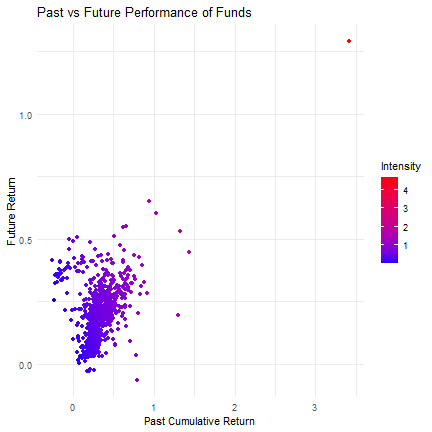
\includegraphics{Question-4_files/figure-latex/Figure 1-1} 

}

\caption{3 year look back scatter plot \label{Figure1}}\label{fig:Figure 1}
\end{figure}

As can be seen from the above graph, there does seem to be a positive
correlation between past cumulative returns and future performance.
However, not so straight forward, as there are some funds that had a
poor past cumulative return but had good future returns. Lets do some
further analysis.

\hypertarget{correlation-analysis-between-cumulative-past-returns-3-years-and-total-flow}{%
\subsubsection{correlation analysis between cumulative past returns (3
years) and total
flow}\label{correlation-analysis-between-cumulative-past-returns-3-years-and-total-flow}}

\begin{verbatim}
## 
##  Pearson's product-moment correlation
## 
## data:  combined_analysis$cumulative_return and combined_analysis$total_flow
## t = 2.038, df = 849, p-value = 0.04186
## alternative hypothesis: true correlation is not equal to 0
## 95 percent confidence interval:
##  0.002581492 0.136338075
## sample estimates:
##        cor 
## 0.06977338
\end{verbatim}

\begin{longtable}[]{@{}cc@{}}
\caption{Correlation Analysis Results}\tabularnewline
\toprule\noalign{}
Statistic & Value \\
\midrule\noalign{}
\endfirsthead
\toprule\noalign{}
Statistic & Value \\
\midrule\noalign{}
\endhead
\bottomrule\noalign{}
\endlastfoot
Correlation Coefficient & 0.0697734 \\
P-Value & 0.0418600 \\
95\% Confidence Interval Lower Bound & 0.0025815 \\
95\% Confidence Interval Upper Bound & 0.1363381 \\
\end{longtable}

The above correlation analysis provides some interesting results. The
output suggests that there is a weak positive relationship between funds
past 3 years performance and fund flows. Thus, although three years past
performance may induce some flows towards that fund this pull is not
relatively strong. Since the p-value is below 0.05 this weak postie
relationship is not random. Therefore, although there is some truth in
saying a 3 year strong performing fund will induce more investment.
there are most probably a lot more factors that goes into the selection
process of investors when deciding where to allocate there funds.

\hypertarget{lets-create-a-linear-regression-to-see-if-3-years-past-performance-does-indicate-future-performance.}{%
\subsection{Lets create a linear regression to see if 3 years past
performance does indicate future
performance.}\label{lets-create-a-linear-regression-to-see-if-3-years-past-performance-does-indicate-future-performance.}}

\begin{verbatim}
## 
## Call:
## lm(formula = future_return ~ cumulative_return, data = combined_analysis)
## 
## Residuals:
##      Min       1Q   Median       3Q      Max 
## -0.35143 -0.08688 -0.01069  0.05119  0.49152 
## 
## Coefficients:
##                   Estimate Std. Error t value Pr(>|t|)    
## (Intercept)       0.130772   0.006873   19.03   <2e-16 ***
## cumulative_return 0.195478   0.017903   10.92   <2e-16 ***
## ---
## Signif. codes:  0 '***' 0.001 '**' 0.01 '*' 0.05 '.' 0.1 ' ' 1
## 
## Residual standard error: 0.1103 on 849 degrees of freedom
##   (119 observations deleted due to missingness)
## Multiple R-squared:  0.1231, Adjusted R-squared:  0.1221 
## F-statistic: 119.2 on 1 and 849 DF,  p-value: < 2.2e-16
\end{verbatim}

\begin{longtable}[]{@{}ccccc@{}}
\caption{Linear Regression Model Summary}\tabularnewline
\toprule\noalign{}
term & estimate & std.error & statistic & p.value \\
\midrule\noalign{}
\endfirsthead
\toprule\noalign{}
term & estimate & std.error & statistic & p.value \\
\midrule\noalign{}
\endhead
\bottomrule\noalign{}
\endlastfoot
(Intercept) & 0.1308 & 0.0069 & 19.0265 & 0 \\
cumulative\_return & 0.1955 & 0.0179 & 10.9190 & 0 \\
\end{longtable}

This regression analysis shows that there is a statistically significant
relationship between past return values and future return values. Thus
funds with higher past returns tend to have higher future returns.
However the R-squared value is fairly low at 0.12 which suggests that
past performance only explain 12\% of the variation in future
performance. Thus although past performance does have a statistically
significant positive relationship with future performance, this
relationship is fairly week and should not be solely relied upon.

\hypertarget{lets-evaluate-the-10-year-look-back-period}{%
\subsection{Lets evaluate the 10 year look back
period}\label{lets-evaluate-the-10-year-look-back-period}}

\hypertarget{calculating-cumulative-returns-for-the-10-year-look-back-period}{%
\subsubsection{Calculating cumulative returns for the 10 year look back
period}\label{calculating-cumulative-returns-for-the-10-year-look-back-period}}

The cumulative returns of the 10 year period is calculated so that a
comparative analysis can be done.

\hypertarget{analyizing-fund-flows-and-future-performance-1}{%
\subsubsection{Analyizing fund flows and future
performance}\label{analyizing-fund-flows-and-future-performance-1}}

Calculating the future performance (the performance a year after the
look back period) will provide somewhat of an answer to whether the look
back period was a good indicating of the following period.

\hypertarget{analyizing-data-1}{%
\subsubsection{Analyizing data}\label{analyizing-data-1}}

To analyze the data, a scatter plot, correlation analysis and regression
analysis will be conducted.

\hypertarget{scatter-plot-illustrating-the-relationship-between-past-performance-and-future-performance-1}{%
\subsubsection{Scatter plot illustrating the relationship between past
performance and future
performance}\label{scatter-plot-illustrating-the-relationship-between-past-performance-and-future-performance-1}}

\begin{figure}[H]

{\centering 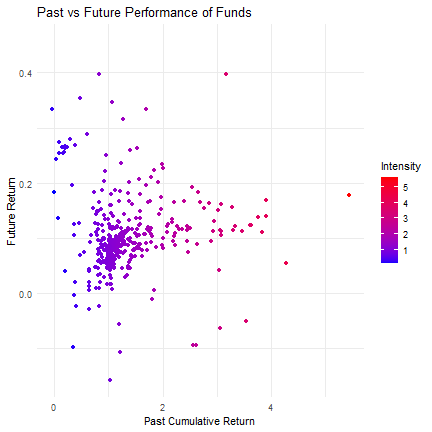
\includegraphics{Question-4_files/figure-latex/Figure 2-1} 

}

\caption{10 year look back scatter plot \label{Figure2}}\label{fig:Figure 2}
\end{figure}

As can be seen from the above figure, there is a far greater variability
when the look back period is increased to 10 years. More importantly
there still seems to be a positive relationship between past cumulative
returns and future returns. However, to identify whether this
relationship is stronger or weaker at longer look back periods we will
have to complete a correlation and regression analysis.

\hypertarget{correlation-analysis-between-cumulative-past-returns-10-years-and-total-flow}{%
\subsubsection{correlation analysis between cumulative past returns (10
years) and total
flow}\label{correlation-analysis-between-cumulative-past-returns-10-years-and-total-flow}}

\begin{verbatim}
## 
##  Pearson's product-moment correlation
## 
## data:  combined_analysis$cumulative_return_10 and combined_analysis$total_flow
## t = 1.7016, df = 400, p-value = 0.08961
## alternative hypothesis: true correlation is not equal to 0
## 95 percent confidence interval:
##  -0.01314346  0.18107861
## sample estimates:
##        cor 
## 0.08477276
\end{verbatim}

\begin{longtable}[]{@{}cc@{}}
\caption{Correlation Analysis Results}\tabularnewline
\toprule\noalign{}
Statistic & Value \\
\midrule\noalign{}
\endfirsthead
\toprule\noalign{}
Statistic & Value \\
\midrule\noalign{}
\endhead
\bottomrule\noalign{}
\endlastfoot
Correlation Coefficient & 0.0847728 \\
P-Value & 0.0896100 \\
95\% Confidence Interval Lower Bound & -0.0131435 \\
95\% Confidence Interval Upper Bound & 0.1810786 \\
\end{longtable}

Like that of the 3 year look back period the correlation between past
performance and funds flow is still weakly positive at 0.08. This is
stronger than that of the three year look back period at 0.07 however it
is not aas strong as I would have thought. Furthermore, the p-value has
increased from 0.04 (for the 3 year look back period) to 0.08 which
suggests that the results are not statistically significant at the 5\%
level. However, these results are still statistically significant at the
10\% level. The main takeaway from this correlation analysis is that by
increasing the look back period we have not increased the correlation
between past fund performance and funds flow.

Lets now have a look at the regression analysis for the 10 year look
back period.

\hypertarget{lets-create-a-linear-regression-to-see-if103-years-past-performance-does-indicate-future-performance.}{%
\subsubsection{Lets create a linear regression to see if103 years past
performance does indicate future
performance.}\label{lets-create-a-linear-regression-to-see-if103-years-past-performance-does-indicate-future-performance.}}

\begin{verbatim}
## 
## Call:
## lm(formula = future_return_10 ~ cumulative_return_10, data = combined_analysis)
## 
## Residuals:
##      Min       1Q   Median       3Q      Max 
## -0.25997 -0.03776 -0.01160  0.01976  0.29579 
## 
## Coefficients:
##                      Estimate Std. Error t value Pr(>|t|)    
## (Intercept)          0.098435   0.007164  13.741   <2e-16 ***
## cumulative_return_10 0.003000   0.004735   0.634    0.527    
## ---
## Signif. codes:  0 '***' 0.001 '**' 0.01 '*' 0.05 '.' 0.1 ' ' 1
## 
## Residual standard error: 0.06966 on 400 degrees of freedom
##   (101 observations deleted due to missingness)
## Multiple R-squared:  0.001002,   Adjusted R-squared:  -0.001495 
## F-statistic: 0.4014 on 1 and 400 DF,  p-value: 0.5267
\end{verbatim}

\begin{longtable}[]{@{}ccccc@{}}
\caption{Linear Regression Model Summary}\tabularnewline
\toprule\noalign{}
term & estimate & std.error & statistic & p.value \\
\midrule\noalign{}
\endfirsthead
\toprule\noalign{}
term & estimate & std.error & statistic & p.value \\
\midrule\noalign{}
\endhead
\bottomrule\noalign{}
\endlastfoot
(Intercept) & 0.0984 & 0.0072 & 13.7406 & 0.0000 \\
cumulative\_return\_10 & 0.0030 & 0.0047 & 0.6335 & 0.5267 \\
\end{longtable}

From the above regression analysis the results provide some interesting
analysis. Like that of the correlation analysis, the regression analysis
states that there is a weak insignificant relationship between past
cumulative returns and future returns. Thus, even if a fund performs
well for 10 years, this is not a solid indicator that the fund will
perform well in the following period. Furthermore, the regression
analysis provides an extremely low r-squared value that suggests that
past performance does not hold a significant explanation in the future
returns of funds.

\hypertarget{summary}{%
\subsubsection{Summary}\label{summary}}

For both the three year and ten year look back periods, past performance
is not a good indicator at both fund flows and future performance. this
suggests that when investors are looking to invest their money they look
at other factors rather than just past performance, which according to
our analysis is the right approach, as past performance is not a good
indicator at future performance.

\newpage

\hypertarget{references}{%
\section*{References}\label{references}}
\addcontentsline{toc}{section}{References}

\hypertarget{refs}{}
\begin{CSLReferences}{0}{0}
\end{CSLReferences}

\hypertarget{appendix}{%
\section*{Appendix}\label{appendix}}
\addcontentsline{toc}{section}{Appendix}

\hypertarget{appendix-a}{%
\subsection*{Appendix A}\label{appendix-a}}
\addcontentsline{toc}{subsection}{Appendix A}

Some appendix information here

\hypertarget{appendix-b}{%
\subsection*{Appendix B}\label{appendix-b}}
\addcontentsline{toc}{subsection}{Appendix B}

\bibliography{Tex/ref}





\end{document}
